% ОБЯЗАТЕЛЬНО ИМЕННО ТАКОЙ documentclass!
% (Основной кегль = 14pt, поэтому необходим extsizes)
% Формат, разумеется, А4
% article потому что стандарт не подразумевает разделов
% Глава = section, Параграф = subsection
% (понятия "глава" и "параграф" из стандарта)
\documentclass[a4paper,article,14pt]{extarticle}

% Подключаем главный пакет со всем необходимым
\usepackage{spbudiploma}

% Пакеты по желанию (самые распространенные)
% Хитрые мат. символы
\usepackage{euscript}
% Таблицы
\usepackage{longtable}
\usepackage{makecell}
% Картинки (можно встявлять даже pdf)
\usepackage[pdftex]{graphicx}

\usepackage{amsthm,amssymb, amsmath}
\usepackage{textcomp}
\usepackage{amsmath}


\begin{document}

% Титульник в файле titlepage.tex
% --------------------- Стандарт СПбГУ для ВКР --------------------------
% Автор: Тоскин Николай, itonik@me.com
% Если заметили ошибку, напишите на email
% Если хотите добавить изменение самостоятельно, GitHub: . PR-s welcome!
% Использованы материалы:
% habr.com/ru/post/144648/
% cpsconf.ru
% Текст:
% http://edu.spbu.ru/images/data/normativ_acts/local/20181030_10432_1.pdf
% Титульный лист:
% http://edu.spbu.ru/images/data/normativ_acts/local/20180703_6616_1.pdf
% -----------------------------------------------------------------------

% Титульный лист диплома СПбГУ
% Временное удаление foot на titlepage
\newgeometry{left=30mm, top=20mm, right=15mm, bottom=20mm, nohead, nofoot}
\begin{titlepage}
\begin{center}
% Первый символ съедается, первым знаком поставлен Ы
\textbf{Санкт--Петербургский}
\textbf{государственный университет}

\vspace{35mm}

\textbf{\textit{\large Ковалев Святослав Сергеевич}} \\[8mm]
% Название
\textbf{\large Выпускная квалификационная работа}\\[3mm]
\textbf{\textit{\large Прогнозирование временных рядов методами машинного обучения}}

\vspace{20mm}
% TODO: Узнать как правильно
Уровень образования: бакалавриат\\
Направление 01.03.02 «Прикладная математика и информатика»\\
«Прикладная математика, фундаментальная информатика и программирование»\\


% Научный руководитель, рецензент
% Сходить в уч отдел и узнать, правильно ли
\begin{flushright}
{Научный руководитель:} \\
% TODO: Узнать кафедру
профессор, кафедра компьютерных технологий \\ и систем, д.ф. - м.н.  Буре~Владимир Мансурович
\end{flushright}
\begin{flushright}
{Рецензент:} \\
% TODO: Узнать кафедру
профессор, кафедра компьютерных технологий \\и систем, д.ф. - м.н.  Буре~Владимир Мансурович
\end{flushright}

\vfill 

{Санкт-Петербург}
\par{2020 г.}
\end{center}
\end{titlepage}
% Возвращаем настройки geometry обратно (то, что объявлено в преамбуле)
\restoregeometry
% Добавляем 1 к счетчику страниц ПОСЛЕ titlepage, чтобы исключить 
% влияние titlepage environment
\addtocounter{page}{1}

% Содержание
\tableofcontents
\pagebreak
\specialsection{Введение}
\documentclass[12pt]{article}
\begin{document}
Hello world!
$Hello world!$ %math mode
\end{document}

Ежедневно на Санкт-Петербургской международной товарно-сырьевой бирже\cite{spimex} ведутся торги различным сырьем: нефтепродукты, нефть, газ, электроэнергия и~т.\,д.
Торги идут сессиями фиксированной длины в каждый будний день. По результатам каждой торговой сессии публикуется отчет с информацией: средневзвешенная цена, лучшая заявка на покупку и продажу, общий объем продаж и другие показатели.
В данной работе рассмотрим прогнозирование средневзвешенной цены по нефтепродуктам на $n$ дней вперед по двум базисам поставки.

\specialsection{Постановка задачи}

Даны временные ряды
\begin{equation}
    {X_{i} = \{x_{i,t}, t=\overline{1,k}\},\quad i=\overline{1,m}},\label{eq:equation}
\end{equation}
где $m$~--- общее количество рядов, а размер всех рядов совпадает и равен $k$.
Цель~--- предсказать значение всех рядов с лагом $n$. Для этого требуется построить такую модель $A(X_i)$, что
\begin{equation}
    A(X_i)=x_{i, k+n}.\label{eq:equation2}
\end{equation}

\par
Данные по временным рядам взяты из открытых источников.
Прогнозируемые временные ряды: АИ-92, АИ-95, дизельное топливо (летнее/межсезонное), мазут, ТС-1. В качестве базиса поставки была выбрана станция Комбинатская. Таким образом, имеем для анализа пять временных рядов. Данные по всем рядам были выгружены с декабря 2015\, г. по август 2020\, г. Предлагается решать задачу методами статистики.

\specialsection{Обзор литературы}

Какой-то обзор литературы


\section{Ненастоящее введение}
\subsection{Мотивация}

Какая-то мотивация

Ненумерованная формула:

\begin{equation}
    \begin{pmatrix} \dot{\varphi}\\ \dot{\theta} \\ \dot{\psi} \end{pmatrix}
    = \begin{pmatrix}
        cos(\theta)cos(\psi) & -sin(\psi) & 0 \\
        cos(\theta)sin(\psi) & cos(\psi)  & 0 \\
        -sin(\theta)         & 0         &  1
    \end{pmatrix}^{-1}
    \begin{pmatrix} \omega_x\\ \omega_y \\ \omega_z \end{pmatrix}.
\end{equation}

Нумерованная формула:

\begin{equation}
    i^2 = -1.
    \label{eq:my_ref}
\end{equation}

Тест ссылки на формулу ~\ref{eq:my_ref}.

Еще немного текста

\subsection{Постановка задачи}

Еще одна постановка задачи

\subsection{Доступные программные средства}

Ниже тестируется очень большая таблица на несколько страниц

\begin{center}
    \begin{longtable}{|p{2cm}|p{3cm}|p{7cm}|p{3cm}|}
    \caption{Заголовок таблицы}\\
    \hline
    1 & 2 & 3 & 4\\ 
    \hline 
    2 & 2 & 3 & 4\\
    \hline
    3 & 2 & 3 & 4\\
    \hline
    4 & 2 & 3 & 4\\
    \hline
    5 & 2 & 3 & 4\\
    \hline
    6 & 2 & 3 & 4\\
    \hline
    7 & 2 & 3 & 4\\
    \hline
    8 & 2 & 3 & 4\\
    \hline
    9 & 2 & 3 & 4\\
    \hline
    10 & 2 & 3 & 4\\
    \hline
    
    
    \end{longtable}
\end{center}


А также тестируется счетчик таблиц, жирные и двойные линии.

\begin{center}
    \begin{longtable}{|p{2cm}||p{3cm}|p{7cm}|p{3cm}|}
    \caption{Заголовок таблицы нумер 2}\\
    \hline
    1 & 2 & 3 & 4\\ 
    \hline
    2 & 2 & 3 & 4\\
    \hline
    3 & 2 & очень жирная ячейка \par с переносом (работаеттт!) & 4\\
    \hline
    4 & 2 & 3 & 4\\
    \hline
    5 & 2 & 3 & 4\\
    \hline
    6 & 2 & 3 & 4\\
    \hline
    7 & 2 & 3 & 4\\
    \hline
    8 & 2 & 3 & 4\\
    \hline
    9 & 2 & 3 & 4\\
    \hline
    10 & 2 & 3 & 4\\
    \hline
    
    
    \end{longtable}
\end{center}


\subsection{Полученные результаты}

Плейн текст

\section{Основная часть раз}

Плейн текст

\pagebreak
\section{Основная часть два: Теория}


\section{Основная часть два: Детали реализации}
\subsection{Расчётная часть}

\section{Анализ экспериментов.}
\begin{figure}[ht]
\begin{center}
\scalebox{0.4}{
   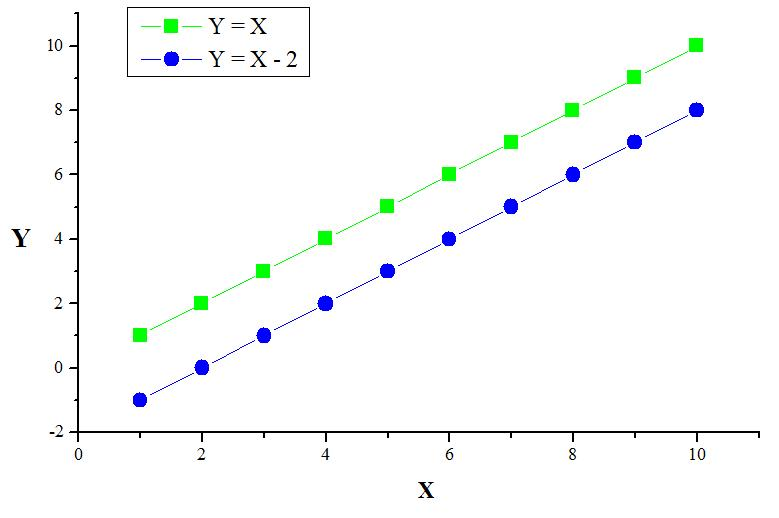
\includegraphics{images/graph.jpg}
}

\caption{
\label{graph-fig}
     Линейные функции.}
\end {center}
\end {figure}
Ссылаемся на график ~\ref{graph-fig}.
Ссылка на статью: ~\cite{voc}, ~\cite{vo2}

\specialsection{Выводы}
Жизнь --- тлен.
\pagebreak

\specialsection{Заключение}

Плейн текст

% Библиография в cpsconf стиле
% Аргумент {1} ниже включает переопределенный стиль с выравниванием слева
\begin{thebibliography}{1}
\bibitem{voc} Griffin D.W., Lim J.S. \flqq Multiband excitation vocoder\frqq. IEEE ASSP-36 (8), 1988, pp. 1223-1235.
\bibitem{vo2} Griffin D.W., Lim J.S. \flqq Multiband excitation vocoder\frqq. IEEE ASSP-36 (8), 1988, pp. 1223-1235.
\end{thebibliography}
\end{document}